% IMP projekt
% Juraj Holub
% xholub40@stud.fit.vutbr.cz

\documentclass[a4paper, 10pt]{article}
\usepackage[utf8]{inputenc}
\usepackage[czech]{babel}
\usepackage[T1]{fontenc}
\usepackage[left=2cm,top=2.5cm, right=2cm]{geometry}
\usepackage{hyperref}
\usepackage{graphicx}
\usepackage{float}

\title{IMP - Mikroprocesorové a vestavěné systémy \\ \medskip\medskip \large{ARM-FITkit3: Stopky na 7-segmentovom displeji}}
\author{Juraj Holub \\xholub40@stud.fit.vutbr.cz}
%\date{}

\begin{document}
	\maketitle
	\thispagestyle{empty}

\section{Úvod}
Táto práca dokumentuje návrh a implementáciu vstavaného softwaru (SW), ktorý realizuje digitáne stopky na 7-segmentovom displeji \footnote{viď dokumentácia led displeju  \href{https://www.gme.cz/data/attachments/dsh.512-924.1.pdf}{https://www.gme.cz/data/attachments/dsh.512-924.1.pdf}} . SW je určený pre mikrokontrolér (MCU) rady \textit{K60} \footnote{viď dokumentácia výrobcu  \href{https://www.nxp.com/part/MK60DN512ZVMD10}{https://www.nxp.com/part/MK60DN512ZVMD10}} . Použité MCU je súčasťou vývojovej a experimentálnej platformy \textit{ARM-FITkit3} \footnote{viď dokumentácia ARM-FITkit3  \href{https://minerva.php5.cz/minerva/minerva.php}{https://minerva.php5.cz/minerva/minerva.php}} . Navrhnuté riešenie umožnuje stopovať čas s presnosťou na $10ms$ a taktiež ukladať medzičas.

\section{Popis ovládania}
Vytvorené riešenie poskytuje funkcionalitu ovládanú nasledujucimi tlačítkami \textit{ARM-FITkit3}:
\begin{itemize}
	\item \textbf{SW5}: Spustenie stopovania času.
	\item \textbf{SW3}: Zastavenie stopovania času. Displej zobrazí odmeraný čas v rozsahu 0 až 99.99 $[sec]$ (prekročenie tohto rozsahu vedie k resetovaniu čítania).
	\item \textbf{SW4}: V čase stopovania umožní ukladať 1 až 4 medzičasi. 
	\item \textbf{SW2}: Po zastavení stopovania prepína medzi zaznamenanými medzičasmi.
	\item \textbf{SW6}: Zmaže namerané hodnoty a vynuluje stopky.
\end{itemize}

\section{Schéma zapojenia}
Keďže led displej nie je súčasťou ARM-FITkit3, bol pripojený na piny poľa \textit{P1} \footnote{ARM-FITkit3 schéma pinov poľa P1 \href{https://minerva.php5.cz/doc/schemata/pg_0007.pdf}{https://minerva.php5.cz/doc/schemata/pg\_0007.pdf}} . Označenie pinov led displeja, jednotlivých diód v rámci jedného panela a označenie jednotlivých panelov popisuje obrázok \ref{led_scheme}. 

\begin{figure}[H] 
	\centering
	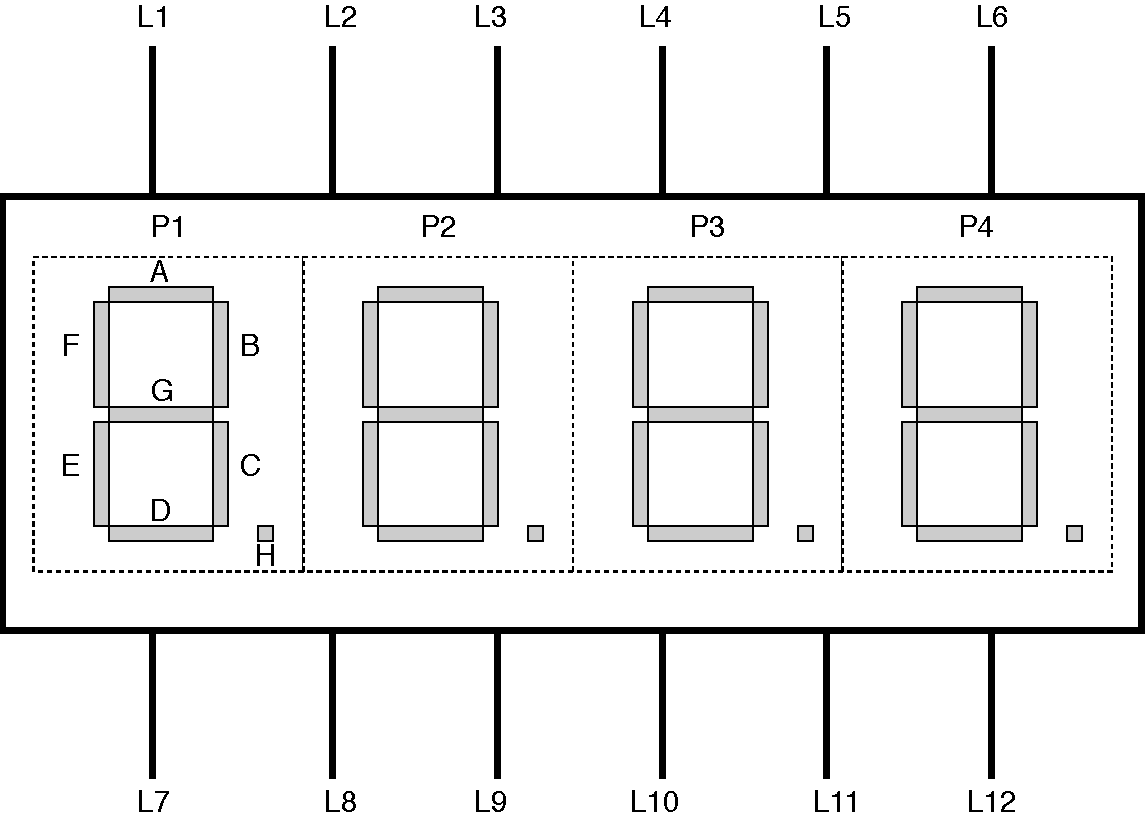
\includegraphics[width=.8\paperwidth]{led_display_scheme.pdf}
	\caption{Schéma pinov led displeja. Označenie led diód v jednom paneli a označenie panelov.}
	\label{led_scheme}
\end{figure}

V tabuľke \ref{tab:map_led_segment} je popísané mapovanie portov led displeja na konkrétne led segmenty. Ak je na zvolenom port logická 0, tak bude daný led segment rozsvietený. 

\begin{table}[H]
	\centering
	\begin{tabular}{|c|c|c|c|c|c|c|c|c|}
		\hline
		\textbf{Led segment} & A & B & C & D & E & F & G & H \\ \hline
		\textbf{Pin} & L2 & L6 & L10 & L8 & L7 & L3 & L11 & L9 \\ \hline
	\end{tabular}
	\caption{Mapovanie led segmentov na piny.}
	\label{tab:map_led_segment}
\end{table}

Mapovanie portov led displeja na konkrétny panel zo segmentami je popísané v tabuľke \ref{tab:map_led_panel}. Led segmenty budú aktívne len v paneloch pre ktoré je na ich pin privedená logická 1.

\begin{table}[H]
	\centering
	\begin{tabular}{|c|c|c|c|c|}
		\hline
		\textbf{Led panel} & P1 & P2 & P3 & P4 \\ \hline
		\textbf{Pin} & L1 & L4 & L5 & L12 \\ \hline
	\end{tabular}
	\caption{Mapovanie led panelov na piny.}
	\label{tab:map_led_panel}
\end{table}

Konrétne hodnoty na piny led displeja sú zasielané z MCU. Mapovanie pinov MCU na piny led displeja popisuje obrázok \ref{mcu_to_led_scheme}.

\begin{figure}[H] 
	\centering
	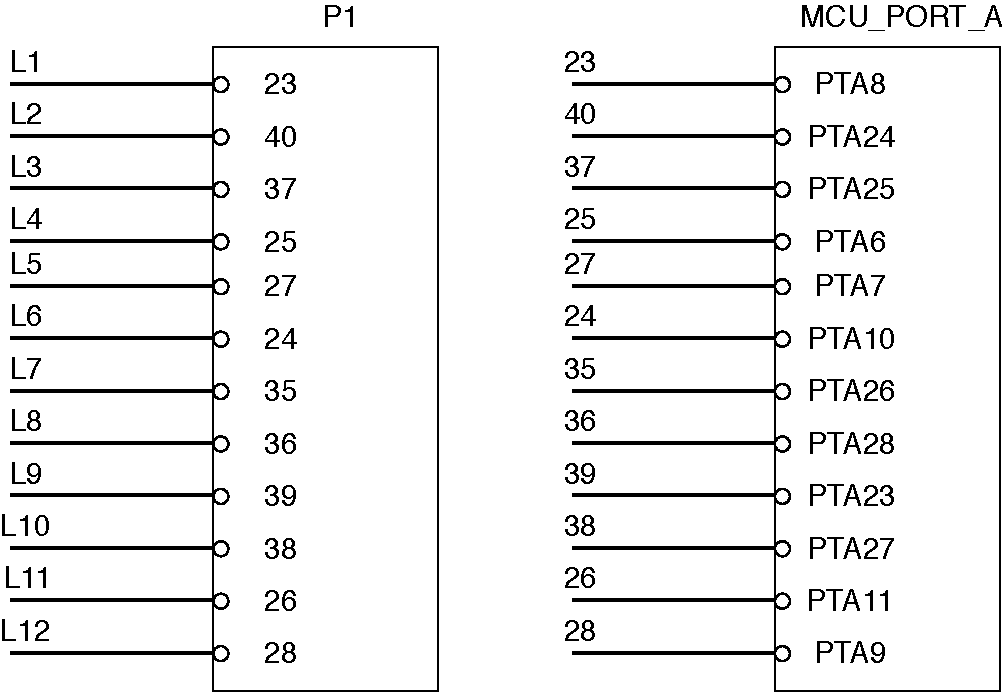
\includegraphics[width=.5\paperwidth]{pin_map_scheme.pdf}
	\caption{Prepojenie pinov led displeja na ARM-FITkit3 pole P1 a prepojenie poľa P1 na MCU piny.}
	\label{mcu_to_led_scheme}
\end{figure}

\section{Implementačné detaily}
Piny mikrokontrolérú, ktoré som využíval patria do skupiny v rámci MCU označenej \textit{Port A}. Pre meranie času som využíval LPTMR0 hodiny (viď dokumentácia MCU), ktoré sa nachádzajú v skupine \textit{Port E}. V tejto skupine sa taktiež nachádzajú tlačítka použité na ovládanie. Tieto dve skupiny boli na MCU aktivované a ostatné skupiny nie. Dôvodom bolo šetrenie spotreby energie, keďže ostatné časti MCU neboli používané.

Jednotka LPTMR0 s generuje prerušenia na frekvencii $1kHz$. V rámci obsluhy prerušenia sa periodicky zasiela z MCU na príslušné porty led displeja výstup, ktorý displej zobrazuje. Keďže zobraziť na displeji je možné vždy len jedno číslo súčasne, tak MCU zasiele postupne v nekonečnom cykle na jednotlivé panely aktuálne hodnoty a to tak rýchlo aby ľudské oko nezbadalo procecs prepínania. Konkrétne hodnoty vypočíta MCU na základe svojich pomocných čítačov, ktoré čítajú podľa potreby na rôznych frekvenciách (počítanie sekúnd, milisekúnd apod.). Referenčná frekvencia pre všetky čítače je $1kHz$ s jednotky LPTMR0. Stalčenie tlačítka vyvolá obsluhu prerušenia, daného tlačítka. 

\section{Záver}
V rámci projektu som sa naučil programovať MCU na základe dokumentácie od výrobcu. Vyskúšal som si pripojenie externých periférií na MCU piny. Možnosti rozšírení vidím v prepojení led displeja s MCU. Napájacie napätie poskytované s MCU v niektorých situáciach nebolo dostatočné vzhľadom na dĺžku prepojovacích vodičov čo viedlo k slabšej viditeľnosti rozsvietených led diód na displeji. Riešením by bolo efektívnejšia (kratšia) prepojovacia sieť.

\end{document}
